% experimental.tex
\documentclass[main.tex]{subfiles}
\begin{document}
\chapter{Experimental Methods} \label{ch:exp}
This chapter explains all the experimental procedures followed to obtain all the parameters necessary to compute the failure surface described by the OOC. This includes detailed information pertaining to the material used, sample geometries and toolpath considerations, as well as describing the equipment used to produce and test the coupons.   

\section{Material} \label{sec:material}

The first step of the experimental work involved development of a custom thermoplastic filament for the FFF process. The reasoning behind this decision was two-fold. First, the use of an off the shelf, commercial thermoplastic filament generally does not guarantee that two different spools were produced under the same processing conditions \textemdash or even using the same parent material. Secondly, the results from Koch \emph{et al.} \cite{Koch2017} show that fluctuations in the filament diameter have an impact in the mechanical properties of FFF parts due to improper volumetric output at the nozzle.

The Cycolac\textregistered~MG94 material produced by SABIC was chosen for this work. This is an Acrylonitrile Butadiene Styrene (ABS) based material traditionally used for injection molding thin walled parts, as well as extrusion of FFF filament. With a reported Melt Flow Index of 11.7 g/10 min, it is an ideal material for both the FFF and extrusion processes. The MG94 was extruded in a setup that consisted of a single screw extruder (Extrudex EDN 45X30D, Germany) with 45 mm screw diameter and L/D ratio of 30D. The hot melt was extruded at 205 $^\circ$C through a circular die with a 5.8 mm diameter, and then guided through a pre-skinner into a vacuum-assisted, heated water bath (Conair, USA) to cool the extrudate whilst minimizing void formation. The solidified filament was then passed through a 3-axis laser micrometer (LaserLinc, USA) and a belt puller (Conair, USA) configured in a control loop. The dimensions of the filament were controlled by automatically adjusting the speed of the puller if the readings from the micrometer were out of specification \textemdash in this case a diameter of 2.85 mm with a tolerance of $\pm$ 0.02 mm. Finally, the product was wound onto spools using a filament winder. A schematic of the extrusion setup can be seen in Figure \ref{fig:extrLine}. Prior to any usage in a printer, the filament was dried in a silo (Novatec, USA) at 82~$^\circ$C for 3 hours.

\begin{figure}[h]
	\center
	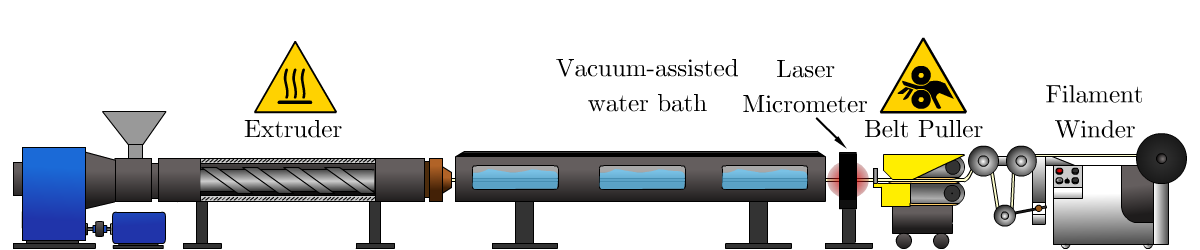
\includegraphics[width=\linewidth]{Extrusion_line}
	\caption{Extrusion line setup} \label{fig:extrLine}
\end{figure}
\pagebreak

\section{Sample Preparation}

As explained in Chapter \ref{ch:oocrit}, the OOC requires mechanical tests to obtain the multiple tensorial components of the mathematical function that describes part failure. Table \ref{tab:testsum} summarizes the tests required.
\begin{table} [h]
\centering
\caption{Mechanical tests required for the OOC}
\begin{tabular}{ c c } 
	\toprule
	\textbf{Mechanical Test} & \textbf{OOC parameters obtained} \\
	\midrule
	Tensile           &   $X_t$, $Y_t$\\
	Compressive       &   $X_c$, $Y_c$\\
	Torsion           &   $S$, $S_{45p}$ , $S_{45n}$\\
	Combined loading  &   $\mu^{1112}$ , $\mu^{2212}$\\
 	\bottomrule
\end{tabular}
\label{tab:testsum}
\end{table}

Given that at the moment of this writing AM testing standards are still in development, custom specimen geometries had to be created in order to test certain loading conditions. Additionally, some bead orientations required are difficult or impossible to reproduce through \emph{2.5-D} FFF. Therefore, the use of a customized robotic, off-axis FFF printer was necessary. This section will detail the coupon geometries used to perform all the mechanical tests described in Table \ref{tab:testsum}, as well as the printing equipment, and toolpath considerations necessary to properly arrange the printed beads in the desired orientation for each condition. 

\subsection{Printing Equipment}
Specimens were produced using either a commercially available desktop FFF printer (Lulzbot TAZ5, USA), or a customized 6-axis robotic printing solution whenever the bead orientation was hard to achieve using a \emph{2.5-D} machine. The robotic printer, developed in the Polymer Engineering Center and nicknamed \emph{Otto} \cite{VanHulle2017}, was based on a 6-axis robot (ABB IRB-120, Switzerland) and fitted with a stationary printhead mounted on an aluminum frame, chosen to be the same extruder from the traditional printer (LulzBot TAZ Single Extruder Tool Head v2, 0.5 mm nozzle, USA) to minimize machine influence on the results. The printing equipment can be seen in Figure \ref{fig:PrintEquip}. 
\begin{figure}[h]
	\center
	\subfloat[TAZ 5 Printer \cite{Lulzbot2018}\label{fig:taz5}]{%
		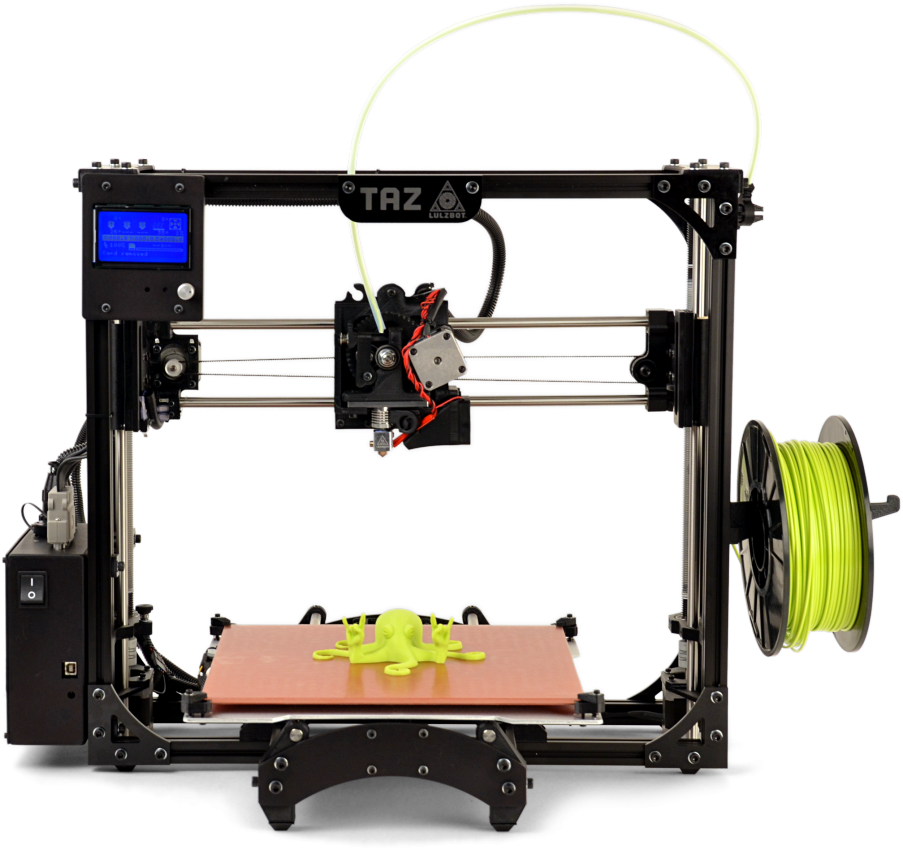
\includegraphics[height=6cm, keepaspectratio]{TAZ_5}
	}
	\hfill
	\subfloat[6-axis robotic printer: \emph{Otto}\label{fig:Otto}]{%
		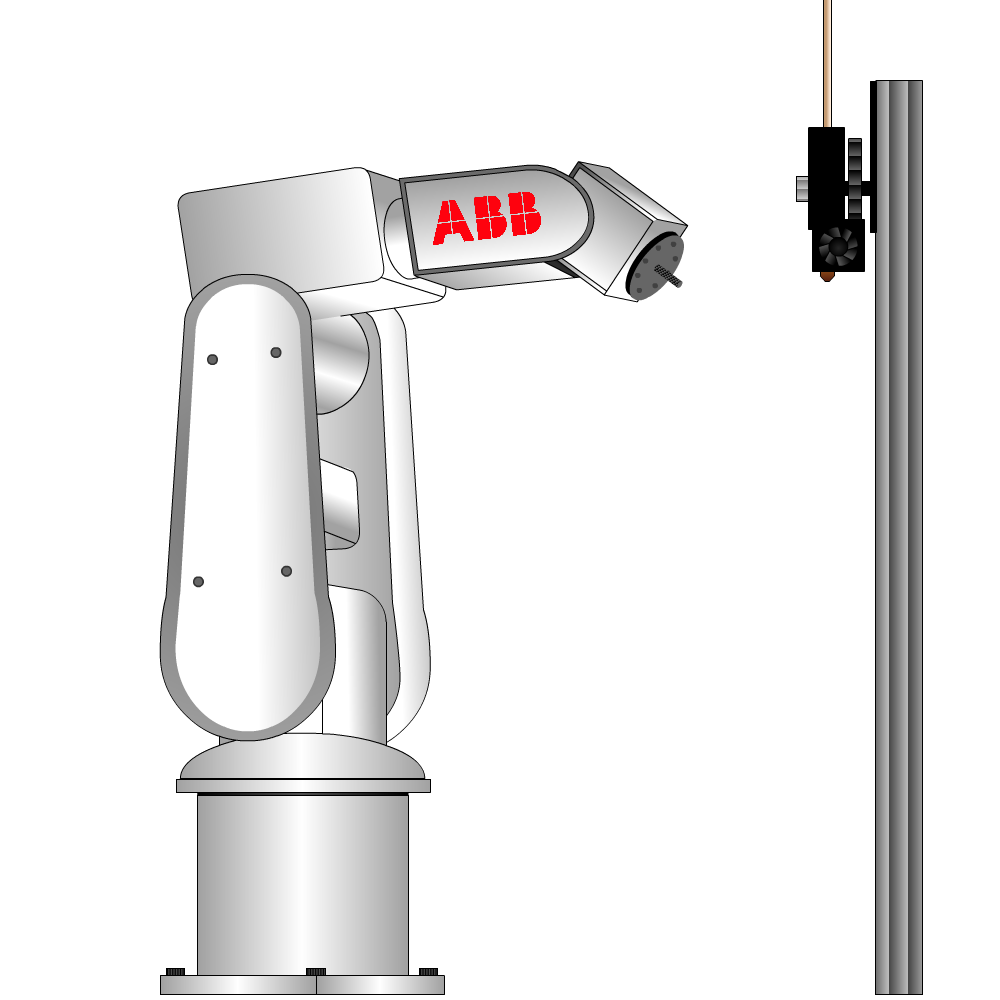
\includegraphics[height=6cm, keepaspectratio]{Otto}
	}
	\caption{Printing equipment} \label{fig:PrintEquip}
\end{figure}

The 6-axis robotic printer's layout is optimized to produce objects of cylindrical nature. A specialized base plate is attached to the sixth axis of the robot, where a threaded rod allows the attachment of disposable plastic cylinders that acts as a build surface. A cylindrical core can then be built by \emph{Otto}, upon which beads in any orientation can be deposited after the robot reorients its joints. Refer to Figure \ref{fig:otto2} for a representation of the process. The left side shows the core being produced atop the disposable build surface, followed by the right hand side, where beads are being laid upon the core in a 45$^\circ$ angle.  
\begin{figure}[h]
	\center
	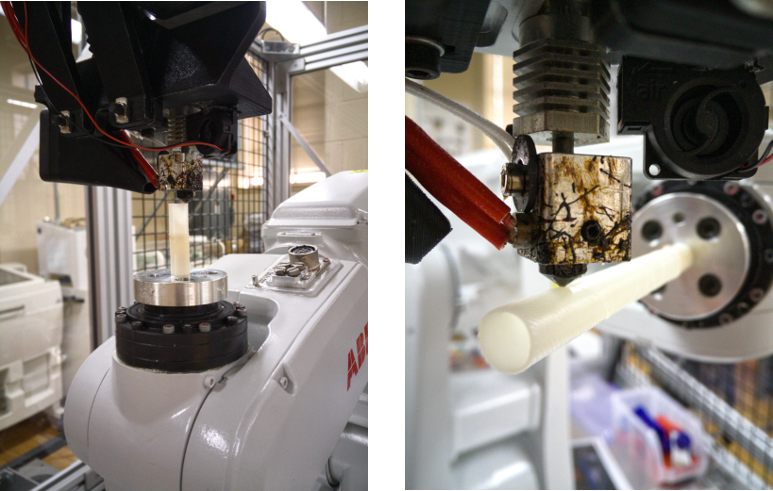
\includegraphics[height=7.5cm, keepaspectratio]{otto2}
	\caption{Print process in \emph{Otto}} \label{fig:otto2}
\end{figure}

Since printing parameters in FFF are known to impact in varying degrees the mechanical performance of objects manufactured through this technology, a conscious effort was made to keep as many processing parameters as possible constant. Table \ref{tab:printparam} summarizes these values.

\begin{table}[!htbp] %Fixates table so that it doesn't randomly jump around between pages
	\renewcommand{\arraystretch}{1.2}
	\centering
	\caption{Constant printing parameters}
	\begin{tabular}{ c c } 
		\toprule
		\textbf{Printing Parameter} & \textbf{Value} \\
		\midrule
		Nozzle temperature & 220$^\circ$C\\
		Bed temperature~\tablefootnote{Applicable only to prints performed on the traditional FFF printer.} & 100$^\circ$C\\
		Printing Speed & 2000 $\frac{mm}{min}$\\
		Layer height & 0.2 mm\\
		Path width & 0.5 mm\\
		Extrusion Factor & 1\\
		\bottomrule
	\end{tabular}
	\label{tab:printparam}
\end{table}

Extrusion Factor (EF) refers to a ratio of the area occupied by the cross section of a bead ($A_{bead}$) divided by the product of the bead width ($W_{bead}$) with the layer height ($H_{layer}$). This factor is used to calculate the length of filament ($L_{fil}$) necessary to produce a bead of known length ($L_{bead}$) as shown in Equations \ref{eq:EFdef} and \ref{eq:EFvol}. The cross sectional area of the filament ($A_{fil}$) is known through the filament diameter used by the printer.

\begin{equation} \label{eq:EFdef}
EF=\frac{A_{bead}}{W_{bead}\times H_{layer}}
\end{equation}  

\begin{equation}\label{eq:EFvol}
\frac{L_{fil}}{L_{bead}}\times A_{fil}=EF \times W_{bead} \times H_{layer}
\end{equation}

   
\subsection{Tensile Specimens}
Tensile coupons were manufactured on the TAZ5, with bead orientations of 0$^\circ$ and 90$^\circ$ with respect to the load direction in order to test $X_t$ and $Y_t$ respectively. The chosen geometry was the ASTM D-638 Type I coupon \cite{ASTMD638} which can be seen in Figure \ref{fig:db}. The toolpath required to produce these samples was developed through \emph{SciSlice}, a customized slicing engine created in the Polymer Engineering Center that allows layer-by-layer and part-by-part controls of crucial process parameters \textemdash such as the bead orientation \textemdash making it ideal for research in the field of FFF \cite{VanHulle2017a}.
\pagebreak
\begin{figure}[h]
	\center
	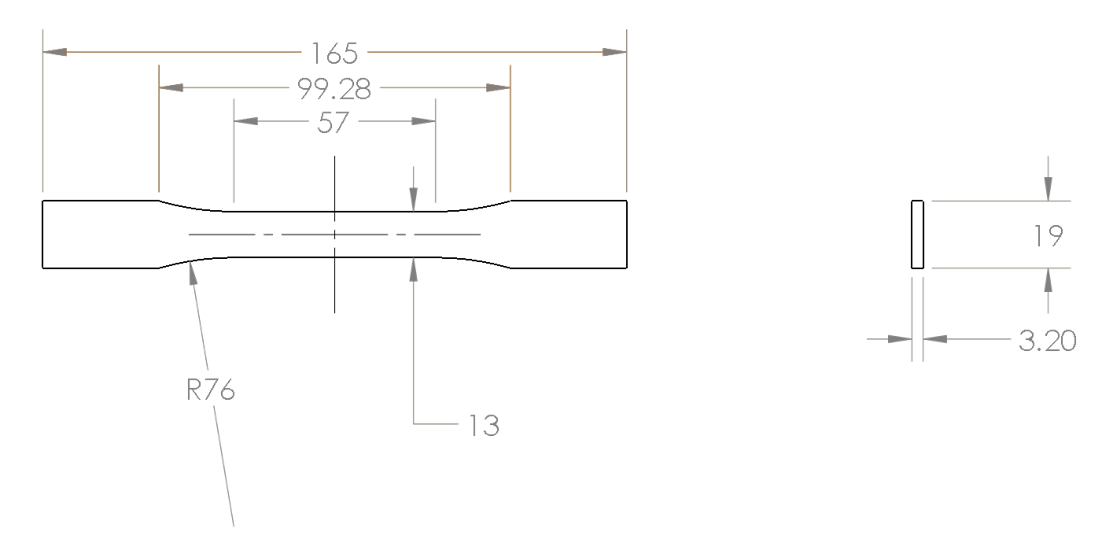
\includegraphics[width=0.95\linewidth, keepaspectratio]{typeIDB}
	\caption{ASTM D-638 Type I coupon} \label{fig:db}
\end{figure}

In order to minimize stress concentrators due to printing discontinuities, the 0$^\circ$ specimens were printed using 13 perimeters, also known as \emph {shells}. This produced a continuous toolpath with beads oriented in the loading direction at the neck section of the specimen. No shells were added to the 90$^\circ$ samples. Refer to Figure \ref{fig:090db} for a visual representation of the coupons. 

\begin{figure}[h]
	\center
	
\includegraphics[width=0.7\linewidth, keepaspectratio]{090db}
	\caption{Toolpath considerations for the tensile coupons} \label{fig:090db}
\end{figure}

\subsection{Compressive Specimens}

Compressive samples were designed with a tubular cross section. This geometry was chosen to mitigate hydrostatic stresses that could artificially increase the compressive strength of the sample if it were made as a completely solid object. Additionally, the cylindrical geometry allowed production of the 0$^\circ$ samples in \emph{Otto}. The geometry can be seen in Figure \ref{fig:comp}.
\begin{figure}[h]
	\center
	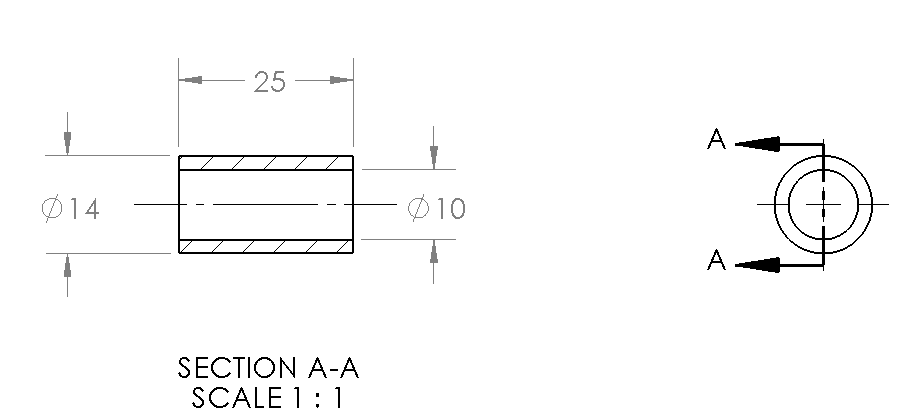
\includegraphics[height=6cm, keepaspectratio]{compres}
	\caption{Compression specimen geometry} \label{fig:comp}
\end{figure}

Compression samples with a bead orientation of 90$^\circ$ with respect to the loading direction were produced using the TAZ5 and \emph{SciSlice}. The coupons with a bead orientation of 0$^\circ$ with respect to the loading direction were made using \emph{Otto} and a customized \emph{Python} script that converted process parameters into instructions for the robotic arm through ABB's \emph{RAPID} toolpathing language. A visual representation of the specimens can be seen in Figure \ref{fig:comp_d}. 
\begin{figure}[h]
	\center
	
\includegraphics[height=5cm, keepaspectratio]{comp_diagram}
	\caption{Representation of compression samples} \label{fig:comp_d}
\end{figure}

\subsection{Torsion and Combined Loading Specimens}

The geometry of the torsion specimens was loosely based in the EN ISO 3167, Type A specimens used by Obst \emph{et al.} \cite{Obst2018}. The cross sectional area of the testing area was chosen to be the same as for the compression specimens. This geometry was chosen since its tubular arrangement allows easy integration with the 6-axis robotic printer, as well as offering axisymmetry and reduction of the risk of artificially increasing the strength of the sample due to yielding restrictions associated with using a completely solid coupon \cite{Obst2018}. However, due to toolpathing complications, more than one torsion geometry was necessary. Each one is described in detail below.  

\subsubsection{45$^\circ$ torsion samples}

To test the $\sigma_{11}$-$\sigma_{22}$ interaction, a torsion sample with beads oriented in 45$^\circ$ was necessary. The geometry, which can be seen in Figure \ref{fig:tors45}, consists of a specimen of cylindrical nature, with a filleted, widening change in cross sectional area that culminates in a gripping section. In this portion, three flat surfaces are added to ensure proper contact with the grips of the torsion machine. 
\begin{figure}[h]
	\center
	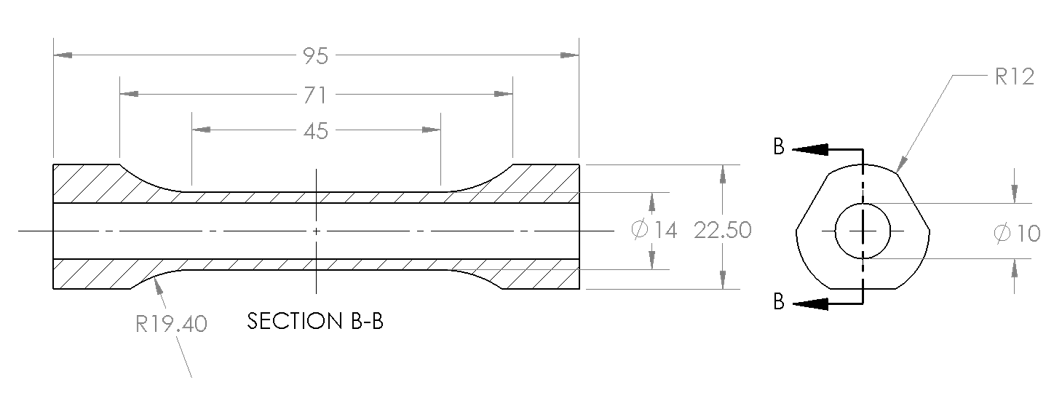
\includegraphics[width=\linewidth, keepaspectratio]{torsion}
	\caption{$S_{45}$ Torsion specimen geometry} \label{fig:tors45}
\end{figure}

The manufacturing of this type of specimen through \emph{Otto} involved laying 10 layers of beads in a 45$^\circ$ angle atop a cylindrical core of 10 mm in diameter and 95 mm in height. Finally, the gripping section is added using beads in alternating  $\pm$45$^\circ$ orientations, culminating in a wider area with a diameter of 24 mm. The flat areas had to be machined in post processing by producing cuts of 1.5 mm in depth in the grips, separated by 120$^\circ$. A visual representation of the finished sample can be seen in Figure \ref{fig:tors45d}. Note that the disposable build surface (visible on the left side of the figure) becomes a part of the coupon without impacting the gage section of the sample. All toolpath was generated using a customized  \emph{Python} script that converted process parameters into instructions for the robotic arm.
\begin{figure}[!htbp]
	\center
	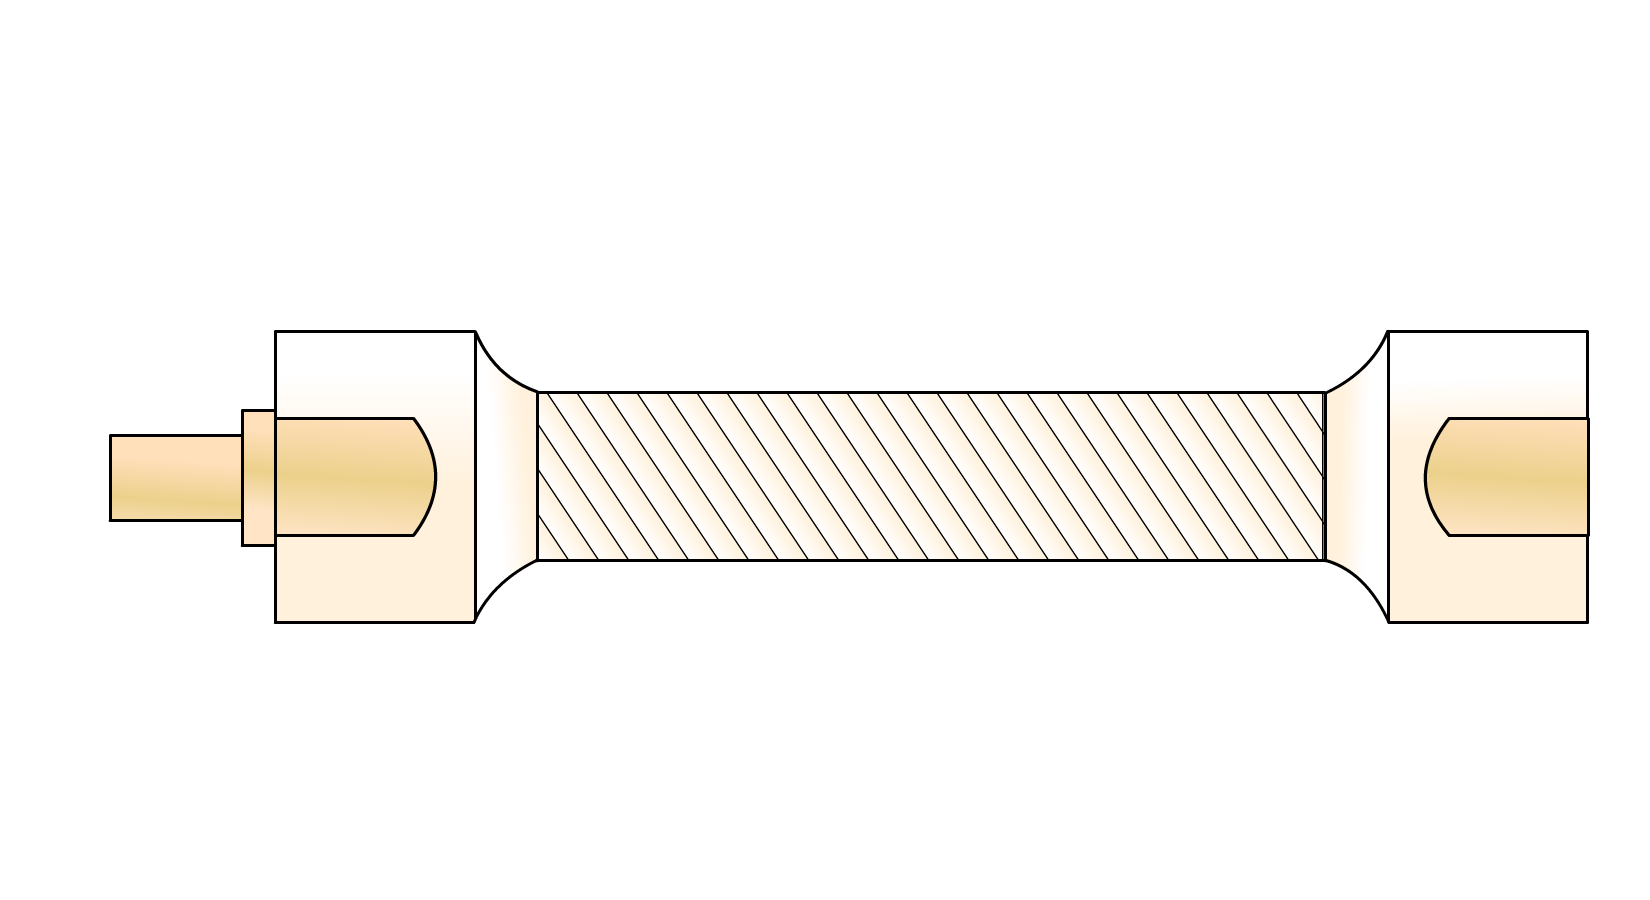
\includegraphics[width=0.35\linewidth, keepaspectratio]{Torsion_45}
	\caption{$S_{45}$ Representation of the 45$^\circ$ specimen} \label{fig:tors45d}
\end{figure}

\subsubsection{0$^\circ$ and 90$^\circ$ torsion samples}
For the 0$^\circ$ and 90$^\circ$ bead orientations, a specimen redesign was necessary due to toolpathing problems. Specifically, the length of the 45$^\circ$ torsion specimens proved problematic to print using 0$^\circ$ and 90$^\circ$ bead orientations, each for different reasons. In the case of the 0$^\circ$ orientation, the long and unidirectional travel distance of each bead introduced considerable tool pressure on the core, causing bowing. This was significant enough to cause poor adhesion of the beads towards the end of the specimen. By contrast, production of 90$^\circ$ samples using the original length caused the sixth axis of the robot to heat up considerably and to almost completely maximize its working range. 

The torsion specimen was redesigned to have the same cross sectional area as the original 45$^\circ$ torsion samples, but shorter length. An optimal distance was devised through multiple print trials where the length of the specimen was varied between 95 and 50 mm. The chosen geometry is shown below in Figure \ref{fig:tors090}.

\begin{figure}[h]
	\center
	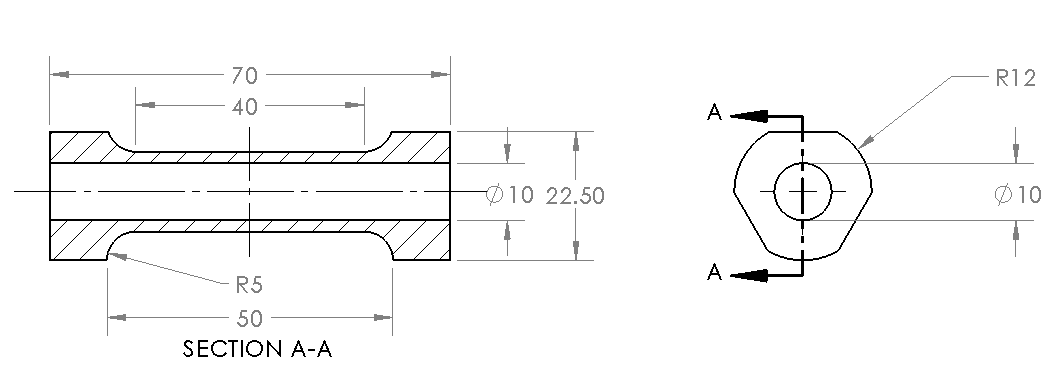
\includegraphics[width=\linewidth, keepaspectratio]{torsion090}
	\caption{Torsion specimen used for 0$^\circ$ and 90$^\circ$ tests} \label{fig:tors090}
\end{figure}

\section{Mechanical Testing}

\subsection{Tension and Compression tests}
Tensile and compressive tests were performed with an Instron 5967 Dual Column Universal testing machine, using a 30 kN load cell. All data acquisition was handled through the accompanying Instron Bluehill 3 software. A movement speed of 5 mm/min was used to deform the 50 mm gage section of the tensile specimens, while a testing speed of 2.5 mm/min was used to deform the 25 mm of height of the compression samples. These testing speeds ensured a strain rate of 0.1 min$^{-1}$ across both specimen types.

The tensile specimens were tested using clamp grips and an extensometer. To protect the samples from excessive gripping force, emery cloth tabs were used, as described by Mazzei Capote \emph{et al}~\cite{Capote2017}. Figure \ref{fig:testsetup} shows a photograph of the setup. Compressive tests were performed using standard compression platens with the universal testing machine. 
    
\subsection{Torsion and Combined loading tests}

All torsion tests were performed using an ADMET eXpert 9618 torsion machine fitted with the MTEST Quattro controller and software suite. The machine sits on a rail system that allows the sample to deform freely during testing. The equipment has two adjustable jaws, with three contact surfaces that holds the sample in place, as shown in Figure \ref{fig:testsetup}. Of the two jaws, one rotates as controlled by a servomotor, while the other is fixed in terms of angular movement. 

\begin{figure}[h]
	\center
	\subfloat[Tensile setup \label{fig:tens}]{%
		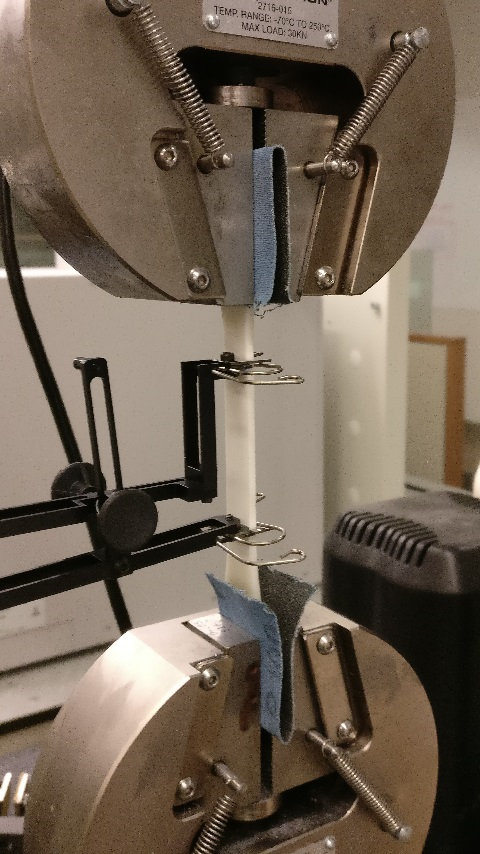
\includegraphics[height=6cm, keepaspectratio]{tensgrip}
	}
	\hfill
	\subfloat[Torsion setup\label{fig:tors}]{%
		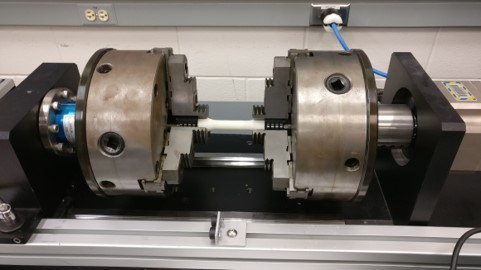
\includegraphics[height=5cm, keepaspectratio]{torsmach}
	}
	\caption{Mechanical testing setup} \label{fig:testsetup}
\end{figure} 

A conscious effort was made to maintain the same strain rate of 0.1 min$^{-1}$ used for the tensile and compression tests. The approach used was the same described by Obst \emph{et al.}~\cite{Obst2018}. The initial assumption is that the shear strain rate ($\dot{\gamma}$) is twice the engineering strain rate ($\dot{\epsilon}$), as shown in Equation \ref{eq:tors1}.

\begin{equation}\label{eq:tors1}
\dot{\gamma}= 2 \times \dot{\epsilon} 
\end{equation}

Figure \ref{fig:torscal} represents a tubular element of outer radius $\rho$ and length L, subjected to a torque T. Using this image as reference, one can see that if point B is fixed in space \textemdash as is the case of the stationary jaw of the torsion machine used throughout this work~\textemdash point A will deform to position A'. The angle of twist $\Phi$ can then be approximated using the arc length $AA'$ as $AA'=\rho \times \Phi$ for small values of shear strain~$\gamma$. It can also be seen in Figure \ref{fig:torscal} that the relationship $AA'=L\times \gamma$ also exists. From this, Equation \ref{eq:tors2} can be obtained.

\begin{figure}[h]
	\center
	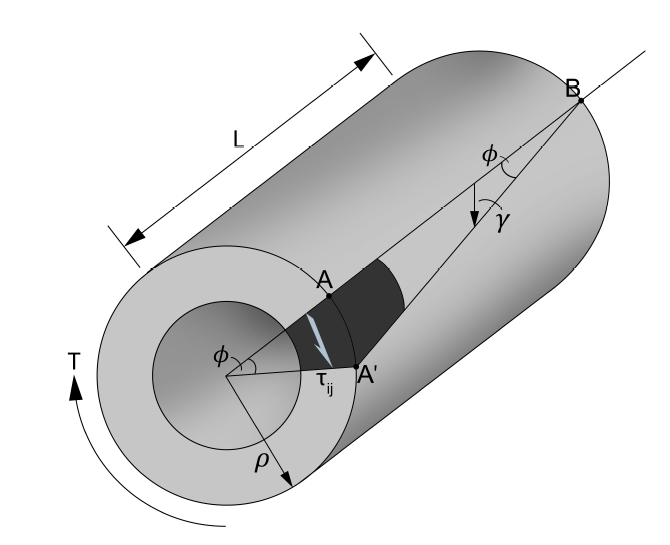
\includegraphics[width=0.55\linewidth, keepaspectratio]{tors2}
	\caption{Stress and strain caused by torque on a tubular geometry~\cite{Obst2018}} \label{fig:torscal}
\end{figure} 

\begin{equation}\label{eq:tors2}
L\times \gamma= \rho \times \Phi  
\end{equation}

Finally, after rearranging and deriving with respect to time, Equation \ref{eq:tors3} is obtained.
\begin{equation}\label{eq:tors3}
\dot{\Phi}=\frac{L\times\dot{\gamma}}{\rho}  
\end{equation}

For this work, $\dot{\gamma}$ is known to be $2 \times 0.1~min^{-1}= 0.2~min^{-1}$, as dictated by Equation \ref{eq:tors1} and the testing conditions chosen for the tensile and compressive tests. In the case of the 45$^\circ$ specimens, preliminary tests performed in positive torsion showed an average outer radius of 6.91 mm and a mean length of failure propagation of 54 mm. Using these values in Equation \ref{eq:tors3} yields a rotational speed of 1.56 rad/min, or 89.4$^\circ$/min. Following a similar procedure for the 0$^\circ$ and 90$^\circ$ samples, the angular speed of the torsion test was calculated, using $L$ as 40 mm, to be 63.7$^\circ$/min.%ELABORATE.

In the case of combined loading scenarios, the setup was fitted with a pulley system that allowed a weight to pull the sample in a nominal direction, while the torsion machine applied shear stresses. Refer to Figure \ref{fig:torscomb} for a visual representation of the compressive and tensile force setup of the torsion machine. 

\begin{figure}[!htbp]
	\center
	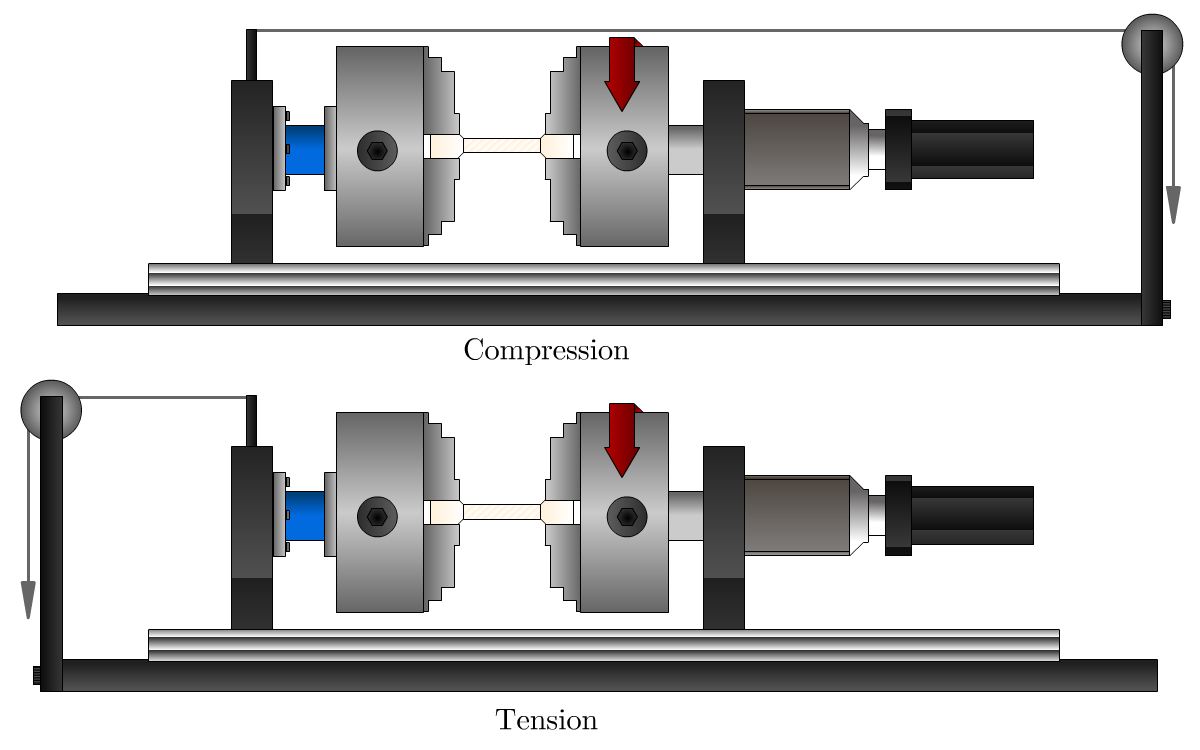
\includegraphics[width=0.8\linewidth, keepaspectratio]{torsion_machine}
	\caption{Machine setup for combined loading scenarios} \label{fig:torscomb}
\end{figure}

The shear stress from the torsion tests was obtained through Equation \ref{eq:shear}, where $\tau_{ij}$, $R$, $T$, and $J_{z}$ represent the shear stress in the $ij$ plane, the outer radius of the test section of the sample, the Torque applied, and the second moment of area respectively.
\begin{equation}\label{eq:shear}
\tau_{ij}=\frac{T\times R}{J_{z}}  
\end{equation}

For this case, the second moment of area is defined as described in Equation \ref{eq:moment}, where $r$ represents the inner radius of the tubular specimen.

\begin{equation}\label{eq:moment}
J_{z}=\frac{\pi\times (R^4-r^4)}{2}  
\end{equation}

Finally, combining Equations \ref{eq:shear} and \ref{eq:moment} yields Equation \ref{eq:shearf}
\begin{equation}\label{eq:shearf}
\tau_{ij}=\frac{2\times T \times R}{\pi\times(R^4-r^4)}  
\end{equation}


Chapter \ref{ch:res} will discuss in detail all results that stem from the experimental methods described. Finally, the failure envelope will be calculated using the mathematical relations described in Chapter \ref{ch:oocrit}.
% Nomenclature introduced in this chapter:
\nomenclature[A]{ABS}{Acrylonitrile Butadiene Styrene}% 
\nomenclature[A]{EF}{Extrusion Factor}%

% Symbols introduced in this chapter:
\nomenclature[S]{$\epsilon$}{Engineering Strain \nomunit{$-$}}%
\nomenclature[S]{$\gamma$}{Shear Strain \nomunit{$-$}}%
\nomenclature[S]{$\dot{\epsilon}$}{Engineering Strain rate \nomunit{$min^{-1}$}}%
\nomenclature[S]{$\dot{\gamma}$}{Shear Strain rate \nomunit{$min^{-1}$}}%
\end{document}